\documentclass[11pt]{article}

\usepackage{verbatim}
\usepackage{setspace}
\usepackage{indentfirst}
\usepackage{algorithm2e}
\usepackage{amsmath, amsthm, graphicx, caption}
\usepackage{float}
\usepackage[margin=1in]{geometry}
\newtheorem{theorem}{Theorem}
\numberwithin{theorem}{subsection}
%\newtheorem{algorithm}[theorem]{Algorithm}
\newtheorem{lemma}[theorem]{Lemma}
\newtheorem{definition}[theorem]{Definition}
\newcommand{\optcost}{\text{Optcost}}
\doublespacing
\title{Keys Under the Welcome Mat \\ 6.857 Final Project Report}
\author{Michelle Wang, Matthew Furtney, Andrew Hyer, Michael Xu}

\begin{document}
\maketitle

\section{Introduction}

The inspiration for this project was a description of a security flaw in Snapchat, published on the internet.\cite{snapchatFlaw1} 
The idea behind the Snapchat application is that pictures sent to and from users will disappear within ten seconds of being opened. 
However, rather than being erased from the device, images are actually stored permanently in device memory unless manually deleted. 

Snapchat uses two methods to prevent users from viewing these images.  First, its UI does not allow them to open these images.  Second,
if a user tries to manually open the image from their disk, they will discover that Snapchat has encrypted it.  Unfortunately, Snapchat
encrypts these images using the encryption key "M02cnQ51Ji97vwT4," which has been hard-coded into the application. Once this key is found 
and known, any user can use it to decrypt these images, accessing images they're not meant to be able to see. We were easily able to find 
this key ourselves in the source code, and thus the idea for our project was born.

With the rapid iteration and agile development style of current software development, new versions of apps get rolled out week to week. With such a fast paced environment, it makes sense that some security may be overlooked and things like hard-coded encryption keys may happen. The purpose of this project was to perform a broad security survey of Android applications as well as a more in-depth look at security vulnerabilities in Snapchat. We would begin by looking for similarly hard-coded encryption strings but expand to look for other security flaws such as the use of depricated algorithms.

\section{Previous Work}

As one may expect, we were not the first to analyze android apks for security vulnerabilities.
Cryptolint was a system designed by researchers at Carnegie Mellon University and the University of California at Santa Barbara to analyze android apps for security vulnerabilities. 
Cryptolint uses software called Androguard for sophisticated static analysis of the decompiled Android apks.
It checks for six specific types of vulnerabilities: 

\begin{enumerate}
  \item ECB mode of block cipher operation
  \item Constant initialization vectors
  \item Constant encryption keys
  \item Static salts for Password-Based Encryption
  \item Fewer than 1000 iterations of Password-Based Encryption
  \item Constant seeds for SecureRandom()
\end{enumerate}

Unfortunately, we could not locate any source code for Cryptolint. Cryptolint's site allows for submission of
applications to be analyzed, but the analyzer did not return any results for us.  Since the source code was unavailable, we could not use or verify any results for ourselves. Moreover, the site only supplies analysis for $5$ apps, 
none of which are very prominent or popular. 

Given these issues, and given our inability to find any other analysis of such apps, we felt justified in designing 
and coding our own analyzer.

\section{Bulk Analysis}

% Assumes a description of the SnapChat vulnerability
  Inspired by Snapchat's snafu, we strove to find similar errors in other popular apps. We downloaded
$917$ popular Android applications in .apk form for analysis. We summarize our method and results below.

\subsection{Implementation}

We downloaded Android APKs from various locations across the Internet, most notably Android Drawer \cite{AndroidDrawer}. Once downloaded, we used
the open-source program APKTool \cite{APKTool} to decompile these APKs. An APK is a zipped compilation of all the executable .dex files that the Android JVM compiles from Java. APKTool decompiles the app into Smali code, which is the language that assembles and disassembles dex files from Java.
We decompiled all $917$ on a single quad-core machine. In addition to the Smali code, this process generated extraneous files
such as images, sound or fonts. 
 
Our next step was to scan the directory and filter the source for relevant strings. We used the Linux utility \texttt{grep} 
to search each directory for lines in Smali files containing ``const-string''. We fed these lines into a Python script
which checked validity based on Shannon entropy, length, and composition (letters and numbers). Before filtering a
decompiled application averaged $200,000$ lines of Smali code. After filtering, we obtained on average only a few dozen
possible hits for each app.

\subsection{Initial Results}

  We manually looked through the lists of \texttt{const-string} objects that our filter had highlighted for our attention.
At first, we focused on searching for purely high-entropy constant strings of significant length. However, a fortunate coincidence 
pointed us down another line of analysis; almost all apps contained hardcoded strings that conveyed information about the type 
of encryption used, along the lines of "SHA1withRSA".  Our filter was quite basic, and so it highlighted these strings as possible 
keys for us.  In light of this discovery, we decided to investigate references to cryptographic algorithms; while seeing that an 
app contains the string ``SHA1withRSA'' does not uncover any actual security flaws, it does tell you something about what encryption 
system the app uses.

\subsection{Aggregate Information}

  Investigating the frequency of cryptographic algorithms yielded some interesting information. We can use
files with a high number of references to pinpoint security hotspots in an application. Additionally, 
cryptographic libraries leave an easily recognizable pattern of crypto references. A quick scan
of our analyzed data reveals that $16$ or $17$ applications make us of the BouncyCastle/SpongyCastle crypto
libraries. The insight here is that we can easily identify which files contains crypto code and check
for hardcoded keys and other vulnerabilities in close proximity.

\subsubsection{Cryptography References}

  Later, we shifted to searching for specific calls to symmetric block cipher methods. We looked for both
block cipher standards and modes such as \textbf{AES}, \textbf{DES}, \textbf{CFB} and \textbf{CBC}. Regex expressions were used to filter
for spurious hits; a string that simply contained \textbf{AES} would not be included. We verified this manually by printing out discovered
references. All the references we inspected were of the format \texttt{AES/CBC/NoPadding} or something similar, which represents
a call to a function from Java's \texttt{Cipher} class in the \texttt{Javax/Crypto} package. Developers who did not use this library for
ciphers may not have been listed, but again our goal was broad trends over a large number of apps. By doing this analysis, we were effectively
examining how a significant proportion of application developers were using block ciphers, and if they were using them correctly.

\begin{figure}[H]
  \caption{References of cryptographic algorithms in $917$ analyzed applications.}
  \centering
  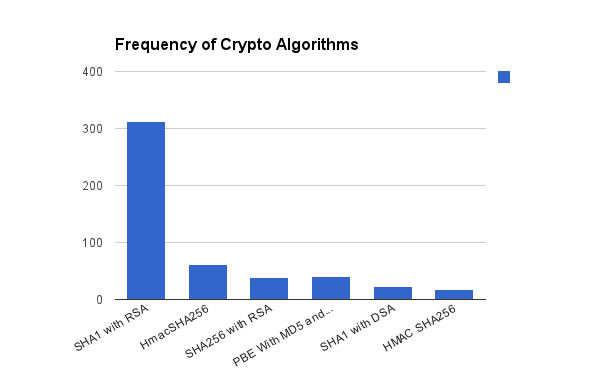
\includegraphics[scale=0.8]{fig1.png}
\end{figure}

\subsubsection{Block Ciphers}

The results we obtained, summarized in Figure 2., are somewhat shocking. We recorded $132$ individual applications which used
\textbf{DES} for their encryption. \textbf{DES} is an antiquated symmetric block cipher standard which relies on $56$ bit keys,
easily brute forceable with modern hardware. While developers may have moives for using \textbf{DES}, in any application that cares
at all about security \textbf{AES} is a far better choice for symmetric block cipher applications. If privacy is at all desired, 
the benefits of secure cryptography far outweight convenience or other justifications. 

We also draw attention to the number of applications that utilize ciphers in \textbf{ECB} mode. For anything more than a single block, 
\textbf{ECB} mode is insecure, since each block will always decrypt in the same way. This essentially leaves the pattern of the 
plaintext intact, leaking significant information. 

(The canonical example of this is \textbf{ECB} mode encryption applied to an image of Tux, the Linux penguin; The encrypted data
clearly reveals the outline of Tux. Any area of uniform color is immediately obvious after \textbf{ECB} encryption.)

We have not uncovered exact details of how these encryption algorithms are being used; when we find an app using ECB mode encryption,
say, we cannot say for certain whether it is using ECB properly (to encrypt a single block of data) or improperly (to encrypt multiple
blocks).  However, our data shows an impressive number of applications that use block ciphers in vulnerable configurations.  We think it
probable that most if not all of these apps are in fact using their configurations improperly, exposing themselves to security risks.

\begin{figure}[H]
  \caption{References of Block Cipher Uses in $917$ analyzed applications.}
  \centering
  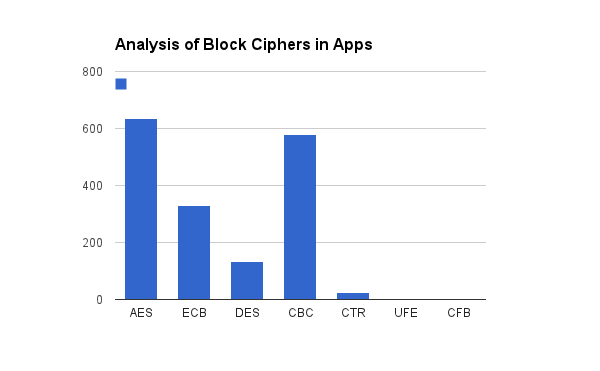
\includegraphics[scale=0.8]{fig2.png}
\end{figure}

\subsection{Back to Snapchat?}

When we ran our basic Python analyzer on Snapchat, we got some interesting results: see Figure 3.

\begin{figure}[H]
  \caption{the output of our filtering algorithm when applied to the decompiled Snapchat code.}
  \centering
  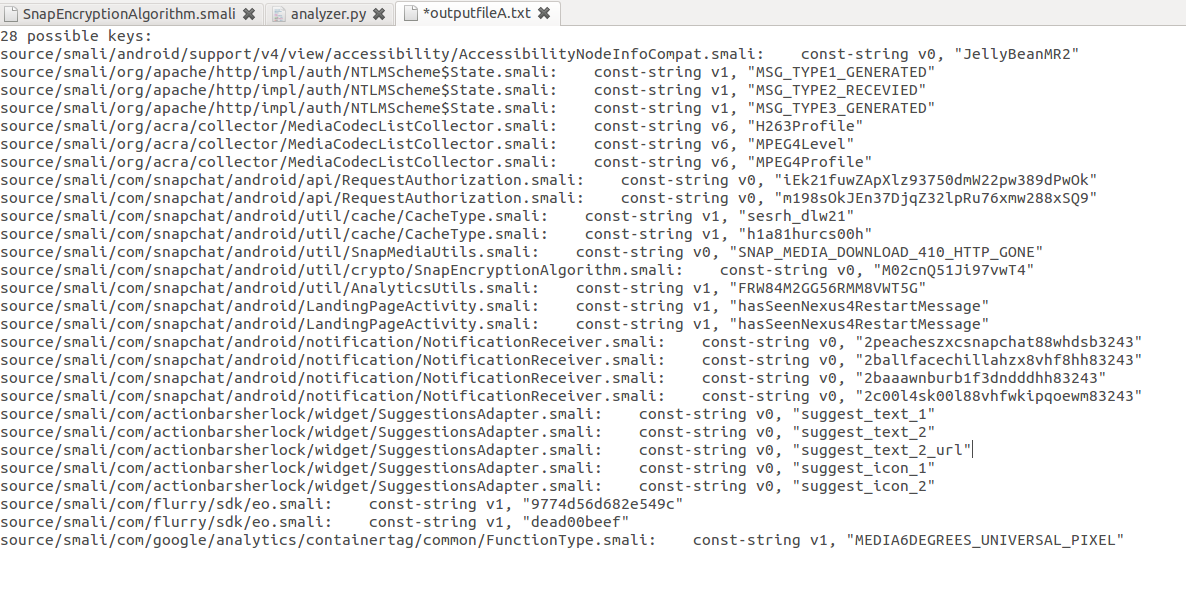
\includegraphics[scale=0.4]{image3.png}
\end{figure}

The key ``M02cnQ51Ji97vwT4'' is, as we would hope, visible here.  However, there are several other sets of
hardcoded strings that look like they could also be keys!  We looked into these, and found some interesting stuff.

There were six keys in the output that looked like they might merit attention:

\begin{itemize}
\item Two strings that look like random keys, in a file called ``RequestAuthorization''. 
\begin{itemize}
\item "iEk21fuwZApXlz93750dmW22pw389dPwOk"
\item "m198sOkJEn37DjqZ32lpRu76xmw288xSQ9"
\end{itemize}
\item Four strings that look like poorly generated passwords, in a file called ``NotificationReciever''.
\begin{itemize}
\item "2peacheszxcsnapchat88whdsb3243"
\item "2ballfacechillahzx8vhf8hh83243"
\item "2baaawnburb1f3dndddhh83243"
\item "2c00l4sk00l88vhfwkipqoewm83243"
\end{itemize}
\end{itemize}

We first Googled these strings to see if they were known of.  The first two keys were: they represent \textbf{another} security
flaw in Snapchat, by which you can access the phone numbers of all Snapchat users and create arbitrary numbers of 'dummy' users.\cite{snapchatFlaw2}

The four strings that looked like poorly done passwords, however, were not found anywhere on the Internet.  We investigated the file
they came from to see if there was anything interesting in there: see Figure 4.

\begin{figure}[H]
  \caption{part of the source code of the file "NotificationReciever", where we found those strange strings}
  \centering
  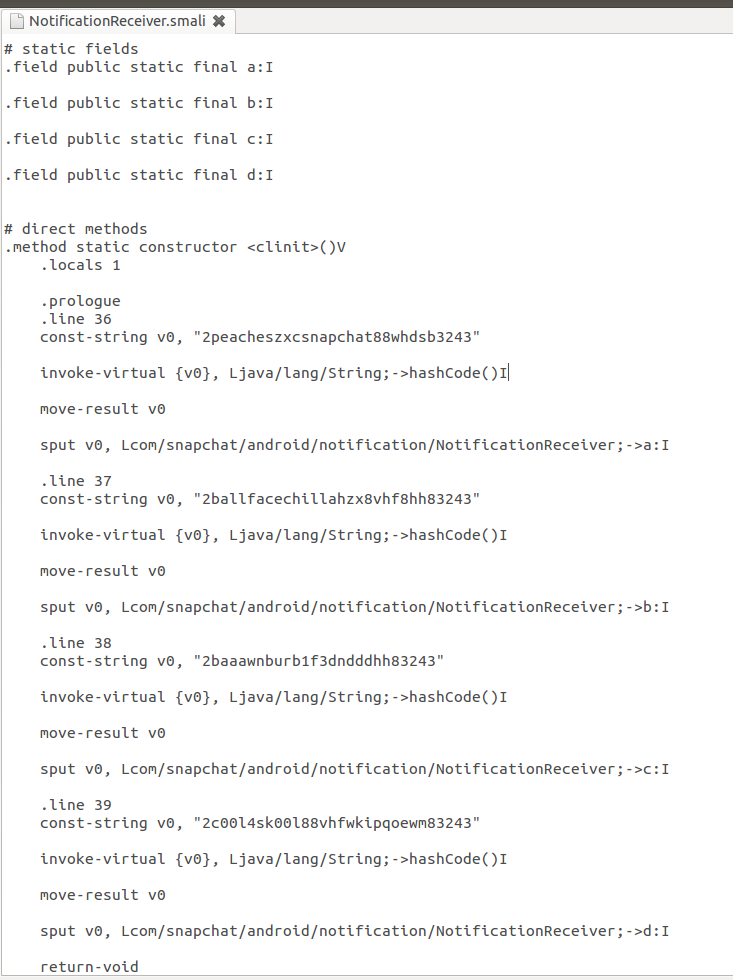
\includegraphics[scale=0.6]{image4.png}
\end{figure}

The code here is in Smali, which is difficult to read, but what's going on on this page is simple enough.  Four integer fields (designated by
letters ``a'' through ``d'' in the decompiled code) are initialized at the top.  Each of the four strings we found is hashed into an int, which 
is inserted into one of those fields.

This means that those integer fields are functionally hard-coded themselves; while their values are recalculated every time, they're recalculated in a
deterministic way from hardcoded inputs, and so will always be the same.  They could represent another flaw in Snapchat.

Unfortunately, none of us understands Smali, and there is no way to reliably decompile Smali into any other language.  This meant that we got rather badly
stuck when trying to explore further into the file and find out what exactly was done with those integer fields.  Nevertheless, we think this is an
interesting line of inquiry, and we hope someone pursues it in future.

\subsection{Continued Investigation}

\subsubsection{Advanced Static Analysis}
  Many of the vulnerabilities discussed in Cryptolint are highly interesting. While the paper describes their methods at a high level, they did not
release any source. Therefore, we plan to extend our analyzer to search for hard-coded or static initialization vectors and seeds. An initialization vector
is the first block passed into a block cipher, it effectively adds a block's worth of random bits to the cipher. A non-random initialization vector
does not provide the security normally guaranteed by a block cipher with a random initialization vector. On a related note, hard-coded seeds,
the input to a pseudo-random number generator, result in deterministic, insecure randomness. Any hard-coded seed used for secure randomness
is a red flag.
  To tackle this slighly deeper analysis, we hope to make use of the same tool the authors of Cryptolint leveraged, Androguard. If Androguard works
as advertised, we should be able to determine when and where a certain variable's value can be manipulated. If there are no opportunities for dynamic modifications
to a variable, we would judge it to be static or hard-coded.

\subsubsection{Dynamic Analysis}

  Another avenue of attack would be to analyze the application during execution. Existing software allows us to intercept the packets sent
and received by the application. This could give us insight into the protocol and allow us to draw more conclusions about the results
obtained by static analysis. Going even further, we could possibly leverage an Android Binary Instrumentation tool, such as \textbf{adbi}. If an
instrumentation tool is effective, it would allow us to inspect variables or data throughout the execution of an application, making it easy
to find deterministic pseudorandomness.

\subsection{Potential Applications}

We think there are a lot of potential future applications to the idea of making users aware of the security (or lack thereof) of apps they use.  We
cannot think of a better example of this than that presented by Snapchat; Snapchat currently has millions of users, who are using it under the
mistaken impression that it provides security.  Given that there are two separate critical security flaws in Snapchat avaiable online (and that
each of them has been online for months or more, with no response from Snapchat), in addition to our own findings, we think that Snapchat's users are being
rather badly misled by Snapchat's claims of 'security'.

\subsection{Conclusion}

Our initial plan was to try to find additional hard-coded encryption keys, and potentially other vunlerabilities.  While our lack of comprehension of Smali
wound up making this extremely difficult, we found another avenue of attack; identifying use of crypto systems with known vulnerabilities.  We found that 
several poor algorithms were used with distressing frequency, meaning that it there are likely vunlerabilities in a fair portion of apps. 

We've suggested a couple lines down which further investigation could go: poking another hole in Snapchat, or analyzing other apps in bulk with some more
sophisticated techniques.  We've also suggested how such information could be brought to the public's attention.

\subsection{Responsible Disclosure: for 6.857 Staff Attention}

When considering vulnerabilities in published software, it is important to be careful not to release anything that will harm software manufacturers.
Through most of our paper, however, we deal with these flaws only in aggregate; we are not mentioning specific apps, only classes of security
flaw that we have observed throughout many apps.  This isn't a significant security issue; these flaws are alread widely known, all we have done is
data gathering to determine how frequent they are.

We have gone into some detail on already-known security flaws of Snapchat.  However, as these flaws are already public knowledge\cite{snapchatFlaw1}\cite{snapchatFlaw2}, 
we do not think it is necessary to contrain the publication of this piece on that basis.

However, there are several aspects of this project that make us leery about releasing this report publicly.  First, our downloading and decompiling
of large numbers of APKs probably violates an equally large number of terms-of-service agreements, and may qualify as software piracy.  Secondly, 
the four strange hashed strings in Snapchat may represent an additional flaw; despite Snapchat's reprehensible behaviour when it comes to fixing 
its security breaches, it would probably be unwise to publish this report without at least making them aware of it in advance.

Overall, this report probably shouldn't be made available on the 6.857 webpage at all, and \textbf{definitely} shouldn't be made public until some time after
Snapchat has been alerted (even though history suggests they are not exactly likely to act on it.) 

\begin{thebibliography}{9}

        \bibitem{snapchatFlaw1}
        http://security.stackexchange.com/questions/52584/why-can-we-still-crack-snapchat-photos-in-12-lines-of-ruby
        \bibitem{snapchatFlaw2}
        http://gibsonsec.org/snapchat/snapchat\_gibsonsec.txt
        \bibitem{APKTool}
        https://code.google.com/p/android-apktool/
        \bibitem{AndroidDrawer}
        http://www.androiddrawer.com/

\end{thebibliography}
\end{document}
